\begin{figure*}
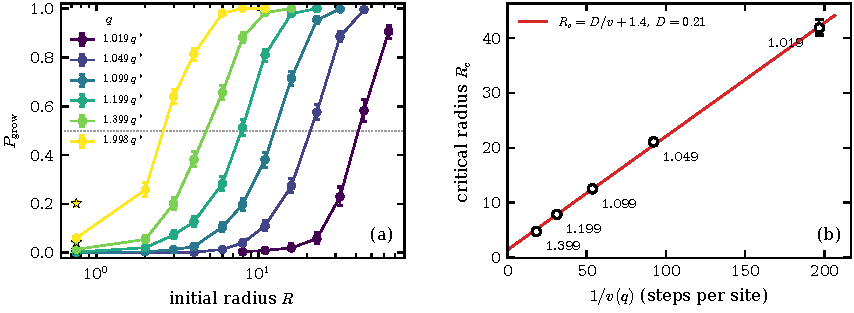
\includegraphics[width=\textwidth]{figs/fig_drop}
\caption{Critical droplets at $p = 1/2$. (a) Probability $P_{\rm grow}$ that a disordered disk of radius $R$
in the dead state reaches the lattice boundary before extinction and before
the declared time horizon, for $q/\qs$ from 1.02 to 2
(500--1000 replicas per point; at $R = 0.75$, a
$2\times2$ block with each site alive with probability $1/2$, 4000 replicas). Stars: the full
$2\times2$ block of live sites (4000 replicas). (b) Radius $R_c$ at
which $P_{\rm grow}=1/2$ against the inverse velocity of a planar front at the same $q$; labels
give $q/\qs$. The line is $R_c=D/v+\Delta R$. Disk protocols use
$L=512$--1024 and horizons $2\times10^4$--$3\times10^5$ depending on $q$;
the $2\times2$ block protocols use $L=1024$, $T=3\times10^4$.
Bars in (a) are 95\% binomial intervals from complete fixed-size replica
ensembles; vertical bars in (b) are conditional bootstrap intervals for the
interpolated $R_c$. The velocities use the corrected outer-envelope tracker.}
\label{fig:drop}
\end{figure*}
